\documentclass[letterpaper,12pt,twoside,]{pinp}

%% Some pieces required from the pandoc template
\providecommand{\tightlist}{%
  \setlength{\itemsep}{0pt}\setlength{\parskip}{0pt}}

% Use the lineno option to display guide line numbers if required.
% Note that the use of elements such as single-column equations
% may affect the guide line number alignment.

\usepackage[T1]{fontenc}
\usepackage[utf8]{inputenc}

% pinp change: the geometry package layout settings need to be set here, not in pinp.cls
\geometry{layoutsize={0.95588\paperwidth,0.98864\paperheight},%
  layouthoffset=0.02206\paperwidth, layoutvoffset=0.00568\paperheight}

\definecolor{pinpblue}{HTML}{185FAF}  % imagecolorpicker on blue for new R logo
\definecolor{pnasbluetext}{RGB}{101,0,0} %


\usepackage{wrapfig,subcaption}

\title{QBUS2820 Assignment 1}

\author[]{}


\setcounter{secnumdepth}{0}

% Please give the surname of the lead author for the running footer
\leadauthor{}

% Keywords are not mandatory, but authors are strongly encouraged to provide them. If provided, please include two to five keywords, separated by the pipe symbol, e.g:
 

\begin{abstract}

\end{abstract}

\dates{This version was compiled on \today} 

% initially we use doi so keep for backwards compatibility
% new name is doi_footer

\pinpfootercontents{QBUS2820 Assignment 1}

\begin{document}

% Optional adjustment to line up main text (after abstract) of first page with line numbers, when using both lineno and twocolumn options.
% You should only change this length when you've finalised the article contents.
\verticaladjustment{-2pt}

\maketitle
\thispagestyle{firststyle}
\ifthenelse{\boolean{shortarticle}}{\ifthenelse{\boolean{singlecolumn}}{\abscontentformatted}{\abscontent}}{}

% If your first paragraph (i.e. with the \dropcap) contains a list environment (quote, quotation, theorem, definition, enumerate, itemize...), the line after the list may have some extra indentation. If this is the case, add \parshape=0 to the end of the list environment.


\hypertarget{introduction}{%
\section{Introduction}\label{introduction}}

\hypertarget{data-processing-and-exploratory-data-analysis}{%
\section{Data processing and exploratory data
analysis}\label{data-processing-and-exploratory-data-analysis}}

\begin{figure}[H]
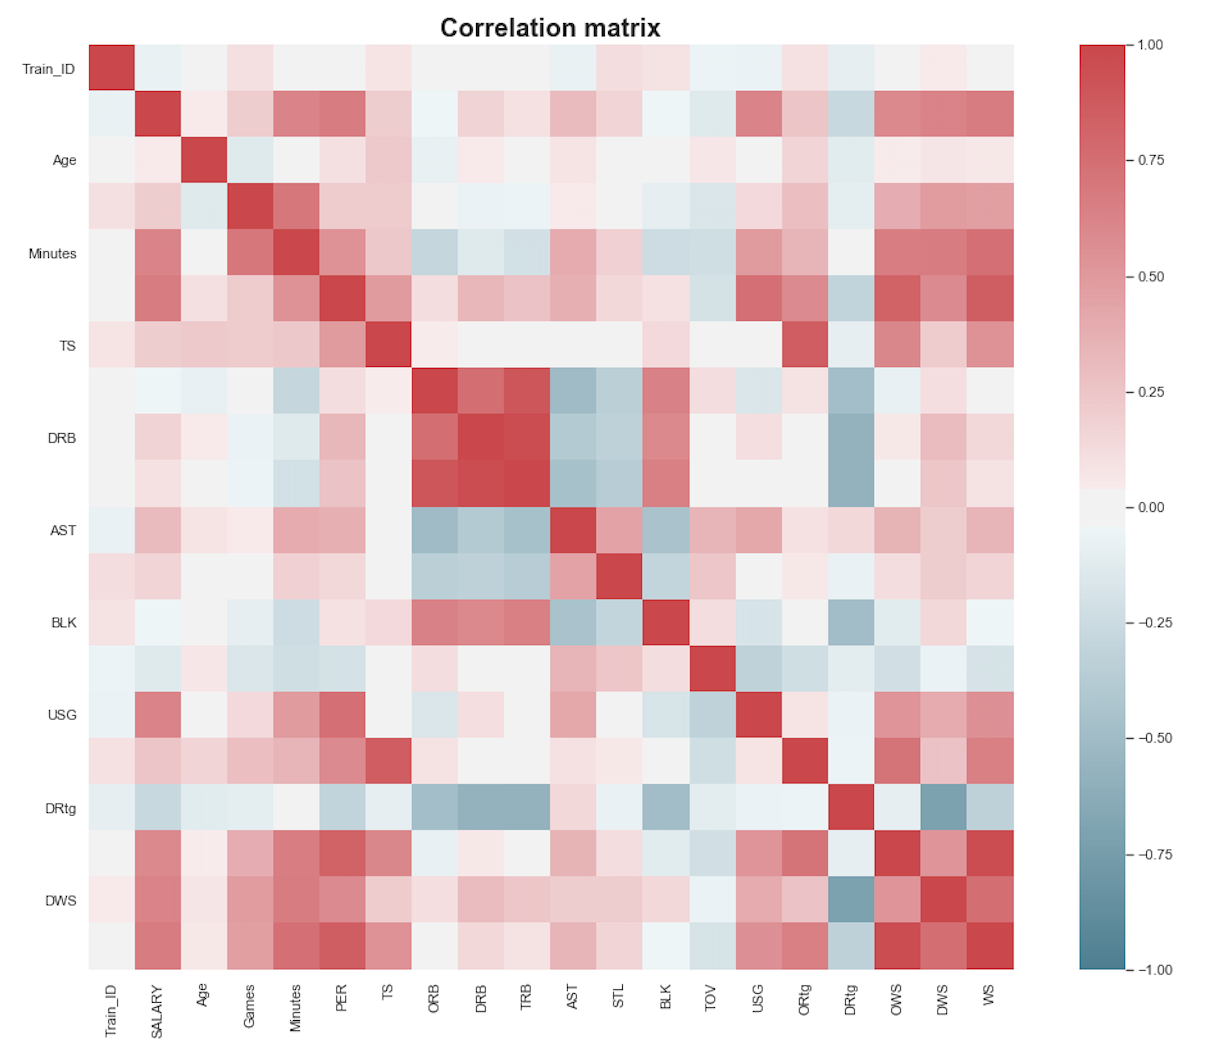
\includegraphics[width=0.8\textwidth]{corr_matrix.png}
\caption{Caption}
\label{fig:figure2}
\end{figure}

\begin{figure}[H]
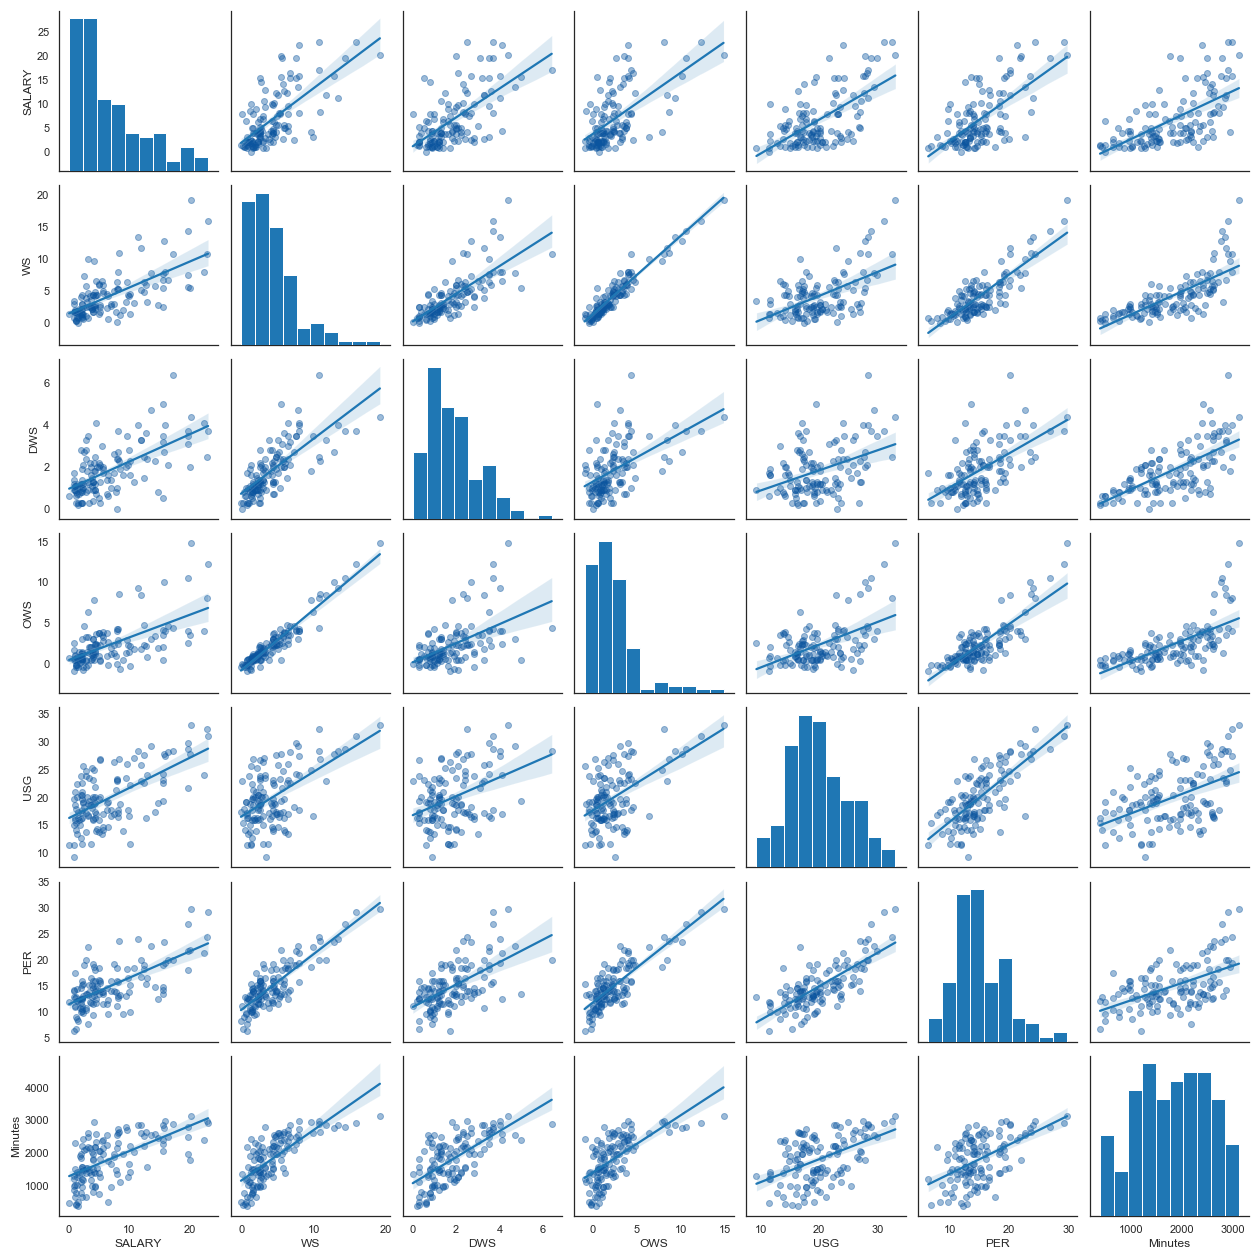
\includegraphics[width=0.8\textwidth]{scatter.png}
\caption{Caption}
\label{fig:figure2}
\end{figure}

\begin{figure}[H]
\begin{subfigure}{0.5\textwidth}
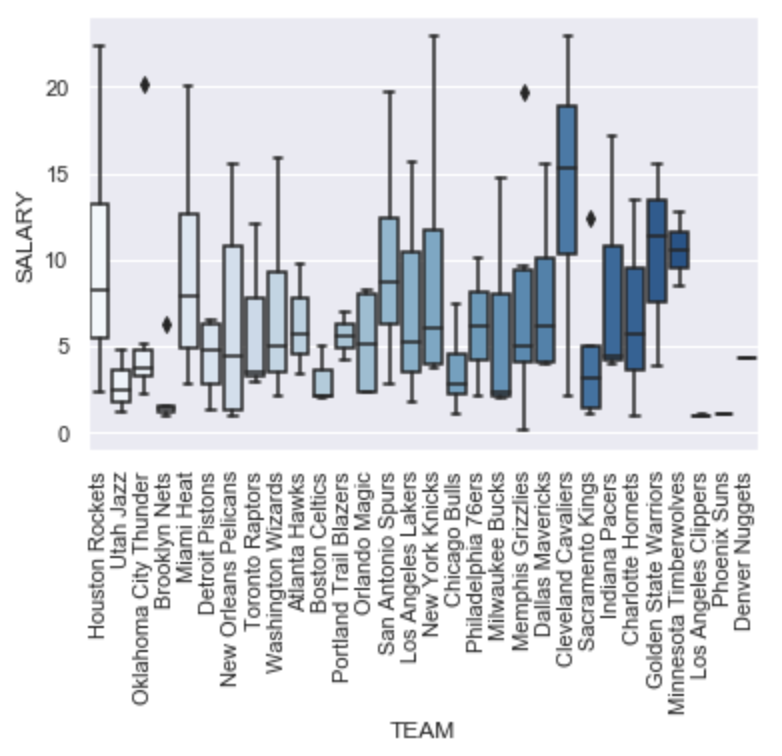
\includegraphics[width=0.9\linewidth, height=5cm]{team_box.png} 
\caption{Salaries for players in different teams.}
\label{fig:subim1}
\end{subfigure}
\begin{subfigure}{0.5\textwidth}
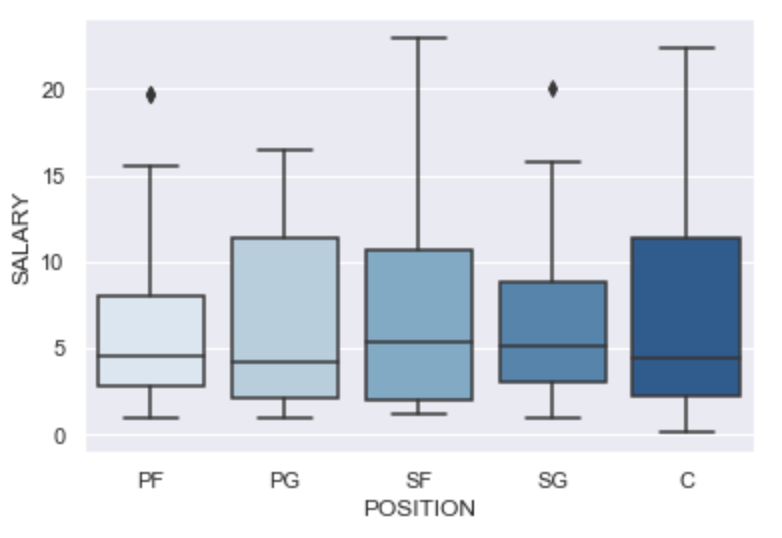
\includegraphics[width=0.9\linewidth, height=5cm]{position_box.png}
\caption{Salaries for players in different positions.}
\label{fig:subim2}
\end{subfigure}
\caption{Boxplots of salaries for players in different teams and positions.}
\end{figure}

As shown in Figuredsgi jsafoisjdf oifj salkadfj oij
lfjsadfisoijfosfijsafdsnglkjgsdifjoasdj dsfjladkfeknwafka

\hypertarget{feature-engineering}{%
\section{Feature engineering}\label{feature-engineering}}

\hypertarget{methodology-of-the-linear-regression-and-knn-regression-models}{%
\section{Methodology of the linear regression and kNN regression
models}\label{methodology-of-the-linear-regression-and-knn-regression-models}}

\begin{figure}[H]
\begin{subfigure}{0.5\textwidth}
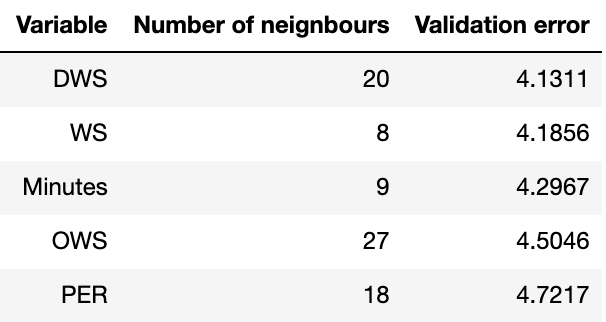
\includegraphics[width=0.9\linewidth, height=5cm]{knn_models.png} 
\caption{Top 5 K nearest neighbbour models with the highest validation errors.}
\label{fig:subim1}
\end{subfigure}
\begin{subfigure}{0.5\textwidth}
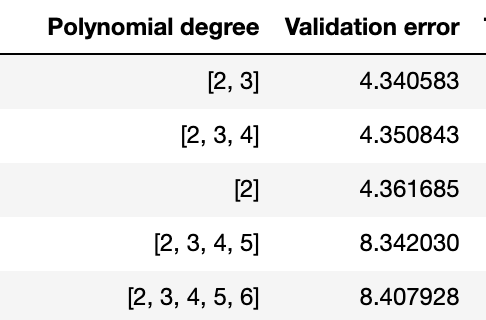
\includegraphics[width=0.9\linewidth, height=5cm]{poly_models.png}
\caption{Top 5 polynomial linear regression models with the highest validation errors.}
\label{fig:subim2}
\end{subfigure}
\caption{Validation errors of 10 models developed.}
\end{figure}

\hypertarget{methodology-of-the-model-that-is-not-covered-in-this-unit}{%
\section{Methodology of the model that is not covered in this
unit}\label{methodology-of-the-model-that-is-not-covered-in-this-unit}}

\hypertarget{test-set-performance}{%
\section{Test set performance}\label{test-set-performance}}

%\showmatmethods


\renewcommand\refname{Analysis and conclusions}
\bibliography{pinp}
\bibliographystyle{jss}



\end{document}

